\documentclass{beamer}

\usepackage{minted}
\setminted{breaklines,python3=true}
\newminted{python}{}
\newminted{pycon}{}
\newcommand{\codepause}{\pause\vspace{-6pt}}

\usepackage{graphicx}


\begin{document}

\begin{frame}
  \frametitle{SciPy}
  \textbf{SciPy} is a set of libraries that basically give Python the ability to mimic MATLAB.
  \begin{itemize}
    \pause
  \item \textbf{SciPy} is also the name of the core numeric library.
    \pause
  \item \textbf{NumPy} provides a fast n-dimensional array type.
    \pause
  \item \textbf{Matplotlib} provides plotting.
    \pause
  \item \textbf{Sympy} provides symbolic computation.
  \end{itemize}
  \pause
  For now, we'll just be talking about NumPy and Matplotlib.
\end{frame}

\begin{frame}[fragile]
  \frametitle{NumPy}
  \inputminted[firstline=1,lastline=3]{pycon}{code/numpy.txt}
  \codepause
  \inputminted[firstline=4,lastline=5]{pycon}{code/numpy.txt}
  \codepause
  \inputminted[firstline=6,lastline=7]{pycon}{code/numpy.txt}
  \codepause
  \inputminted[firstline=8,lastline=9]{pycon}{code/numpy.txt}
\end{frame}

\begin{frame}
  \frametitle{Arrays vs Lists}
  Compared to Python lists, NumPy arrays
  \begin{itemize}
    \pause
  \item are faster,
    \pause
  \item are more memory-efficient,
    \pause
  \item can be broadcasted, and
    \pause
  \item can have multiple dimensions.
  \end{itemize}
  \pause
  However, the dimensions of a NumPy array are fixed from creation. In particular, you cannot append to an array.
\end{frame}

\begin{frame}[fragile]
  \frametitle{\texttt{arange}; Broadcasting}
  \inputminted[firstline=1,lastline=2]{pycon}{code/arange.txt}
  \codepause
  \inputminted[firstline=3,lastline=4]{pycon}{code/arange.txt}
  \codepause
  \inputminted[firstline=5,lastline=6]{pycon}{code/arange.txt}
  \codepause
  \inputminted[firstline=7,lastline=7]{pycon}{code/arange.txt}
  \codepause
  \inputminted[firstline=8,lastline=8]{pycon}{code/arange.txt}
  \codepause
  \inputminted[firstline=9,lastline=11]{pycon}{code/arange.txt}
\end{frame}

\begin{frame}[fragile]
  \frametitle{\texttt{shape}; \texttt{reshape}}
  \inputminted[firstline=1,lastline=2]{pycon}{code/shape.txt}
  \codepause
  \inputminted[firstline=3,lastline=4]{pycon}{code/shape.txt}
  \codepause
  \inputminted[firstline=5,lastline=9]{pycon}{code/shape.txt}
  \codepause
  \inputminted[firstline=10,lastline=11]{pycon}{code/shape.txt}
\end{frame}

\begin{frame}[fragile]
  \frametitle{Multiplication}
  \inputminted[firstline=1,lastline=3]{pycon}{code/matmul.txt}
  \codepause
  \inputminted[firstline=4,lastline=6]{pycon}{code/matmul.txt}
  \codepause
  \inputminted[firstline=7,lastline=7]{pycon}{code/matmul.txt}
  \codepause
  \inputminted[firstline=8,lastline=9]{pycon}{code/matmul.txt}
\end{frame}

\begin{frame}[fragile]
  \frametitle{Matrix Multiplication}
  \inputminted[firstline=10,lastline=12]{pycon}{code/matmul.txt}
  \codepause
  \inputminted[firstline=13,lastline=14]{pycon}{code/matmul.txt}
  \codepause
  \inputminted[firstline=15,lastline=16]{pycon}{code/matmul.txt}
\end{frame}

\begin{frame}[fragile]
  \frametitle{More Broadcasting}
  \inputminted[firstline=1,lastline=5]{pycon}{code/broadcasting.txt}
  \codepause
  \inputminted[firstline=6,lastline=10]{pycon}{code/broadcasting.txt}
\end{frame}

\begin{frame}[fragile]
  \frametitle{More Broadcasting}
  \inputminted[firstline=11,lastline=12]{pycon}{code/broadcasting.txt}
  \codepause
  \inputminted[firstline=13,lastline=17]{pycon}{code/broadcasting.txt}
\end{frame}

\begin{frame}[fragile]
  \frametitle{More Broadcasting}
  \inputminted[firstline=18,lastline=19]{pycon}{code/broadcasting.txt}
  \codepause
  \inputminted[firstline=20,lastline=20]{pycon}{code/broadcasting.txt}
  \codepause
  \inputminted[firstline=21,lastline=23]{pycon}{code/broadcasting.txt}
\end{frame}

\begin{frame}
  \frametitle{Broadcasting Rules}
  Two dimensions are \emph{compatible} when
  \pause
  \begin{itemize}
  \item they have the same size, or
    \pause
  \item at least one of them is \(1\).
  \end{itemize}
  \pause
  Two arrays (or array-like objects) can be used in a single binary operation if all of their dimensions are compatible.
  \pause
  If one array (or array-like object) has fewer dimensions than another, then it is treated as though it had extra dimensions of size \(1\) on the \emph{left} of its shape.
\end{frame}

\begin{frame}[fragile]
  \frametitle{Broadcasting}
  \inputminted[firstline=24,lastline=28]{pycon}{code/broadcasting.txt}
  \codepause
  \inputminted[firstline=29,lastline=33]{pycon}{code/broadcasting.txt}
\end{frame}

\begin{frame}[fragile]
  \frametitle{Transposing; n-dimensional indexing; views}
  \inputminted[firstline=1,lastline=4]{pycon}{code/transpose.txt}
  \codepause
  \inputminted[firstline=5,lastline=8]{pycon}{code/transpose.txt}
  \codepause
  \inputminted[firstline=9,lastline=12]{pycon}{code/transpose.txt}
  \codepause
  \inputminted[firstline=13,lastline=13]{pycon}{code/transpose.txt}
  \codepause
  \inputminted[firstline=14,lastline=16]{pycon}{code/transpose.txt}
\end{frame}

\begin{frame}[fragile]
  \frametitle{More Indexing}
  \inputminted[firstline=1,lastline=5]{pycon}{code/indexing.txt}
  \codepause
  \inputminted[firstline=6,lastline=7]{pycon}{code/indexing.txt}
  \codepause
  \inputminted[firstline=8,lastline=9]{pycon}{code/indexing.txt}
  \codepause
  \inputminted[firstline=10,lastline=12]{pycon}{code/indexing.txt}
  \codepause
  \inputminted[firstline=13,lastline=14]{pycon}{code/indexing.txt}
\end{frame}

\begin{frame}[fragile]
  \frametitle{Comparison}
  \inputminted[firstline=1,lastline=4]{pycon}{code/comparison.txt}
  \codepause
  \inputminted[firstline=5,lastline=5]{pycon}{code/comparison.txt}
  \codepause
  \inputminted[firstline=6,lastline=8]{pycon}{code/comparison.txt}
  \codepause
  \inputminted[firstline=9,lastline=10]{pycon}{code/comparison.txt}
  \codepause
  \inputminted[firstline=11,lastline=11]{pycon}{code/comparison.txt}
  \codepause
  \inputminted[firstline=12,lastline=15]{pycon}{code/comparison.txt}
\end{frame}

\begin{frame}
  \frametitle{Some Useful Functions}
  \begin{itemize}
  \item \texttt{numpy.hstack()}: concatenate arrays horizontally.
  \item \texttt{numpy.vstack()}: concatenate arrays vertically.
  \item \texttt{numpy.zeros()}: create an array of zeros (with a given shape).
  \item \texttt{numpy.ones()}: create an array of ones (with a given shape).
  \item \texttt{numpy.squeeze()}: eliminate length-one dimensions.
  \item \texttt{numpy.ravel()}: flatten an array.
  \item \texttt{numpy.copy()}: copy an array.
  \end{itemize}
\end{frame}

\begin{frame}[fragile]
  \frametitle{Surface Plotting}
  \inputminted[firstline=1,lastline=7]{pycon}{code/plot.txt}
\end{frame}

\begin{frame}[fragile]
  \frametitle{Surface Plotting}
  \inputminted[firstline=8,lastline=8]{pycon}{code/plot.txt}
  \codepause
  \inputminted[firstline=9,lastline=9]{pycon}{code/plot.txt}
  \codepause
  \inputminted[firstline=10,lastline=12]{pycon}{code/plot.txt}
  \codepause
  \inputminted[firstline=13,lastline=13]{pycon}{code/plot.txt}
  \codepause
  \inputminted[firstline=14,lastline=15]{pycon}{code/plot.txt}
\end{frame}

\begin{frame}[fragile]
  \frametitle{Surface Plotting}
  \inputminted[firstline=16,lastline=16]{pycon}{code/plot.txt}
  \codepause
  \inputminted[firstline=17,lastline=17]{pycon}{code/plot.txt}
  \codepause
  \inputminted[firstline=18,lastline=18]{pycon}{code/plot.txt}
  \codepause
  \inputminted[firstline=19,lastline=19]{pycon}{code/plot.txt}
\end{frame}

\begin{frame}
  \centerline{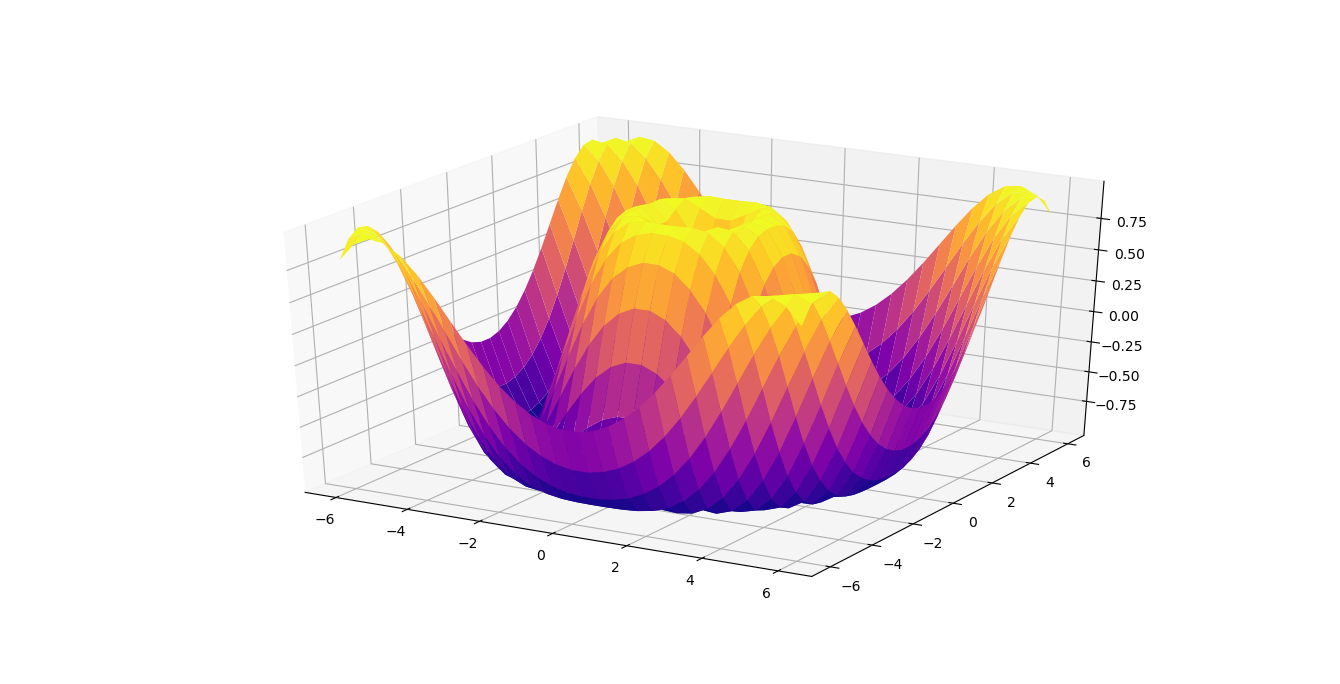
\includegraphics[scale=0.5]{image/plot_surface.png}}
\end{frame}

\begin{frame}
  \frametitle{Exercise: The Fibonacci Sequence}
  The \emph{Fibonacci sequence} is defined by
  \begin{align*}
    F_0 &= 0,
    \\
    F_1 &= 1,
    \\
    F_{n} &= F_{n-2} + F_{n-1} .
  \end{align*}
  Write a function that returns the first \emph{n} Fibonacci numbers.
\end{frame}

\begin{frame}[fragile]
  \frametitle{Example Solution}
  \inputminted[firstline=1,lastline=7]{python}{code/fibonacci.txt}
\end{frame}

\end{document}

%%% Local Variables:
%%% TeX-command-extra-options: "-shell-escape"
%%% End:
